\question ( )有利于CPU繁忙型的作业,而不利于I/O繁忙型的作业(进程)
\par\twoch{时间片轮转调度算法}{\textcolor{red}{先来先服务调度算法}}{短作业(进程)优先调度算法}{优先权调度算法}
\begin{solution}目前存在着多种调度算法,有的算法适用于作业调度,有的算法适用于进程调度;但也有些调度算法既可用于作业调度,也可用于进程调度。其中,先来先服务(FCFS)调度算法是一种最简单的调度算法。FCFS算法比较有利于长作业(进程),而不利于短作业(进程)。FCFS调度算法有利于CPU繁忙型的作业,而不利于I/O繁忙型的作业(进程)。CPU繁忙型作业,是指该类作业需要大量的CPU时间进行计算,而很少请求I/O。通常的科学计算便属于CPU繁忙型作业。I/O繁忙型作业是指CPU进行处理时,又需频繁地请求I/O,而每次I/O的操作时间却很短,目前大多数的事务处理都属于I/O繁忙型作业。
\end{solution}
\question 下面对于剥夺式系统的说法正确的是
\par\fourch{\textcolor{red}{若系统采用时间片轮转调度进程,则系统采用的是剥夺式调度}}{若由于某种事件引起调度,则该系统是剥夺式调度}{实时系统通常采用剥夺式调度}{在剥夺式系统中,进程的周转时间较之非剥夺式系统可预见}
\begin{solution}时间片轮转调度算法是一种剥夺式的调度算法,当时间片用完时,即使当前进程没有执行完,系统也会剥夺当前进程的处理机给下一个进程,A选项正确。
因为某种事件而引起调度,不能确定是否剥夺,有可能是不剥夺系统。只有进程本身等待某事件时才主动放弃处理机而引起调度,才有可能是剥夺系统。采用优先级剥夺调度策略,当有优先级更高的进程到达时,会剥夺当前进程处理机并引起调度,因此B选项错误。
实时系统是否剥夺是不确定的,如订票系统通常不会采用剥夺策略,不然会导致被剥夺的用户购票失败,C选项错误。
剥夺式系统中,进程的执行顺序不可预知,因此无法估算周转时间,相反非剥夺的系统会由于调度顺序可预见而使周转时间更容易预见,D选项错误。
\end{solution}
\question 有5个批处理作业几乎同时到达,其预计运行时间分别为10、6、2、4、8,其优先级(由外部设定)分别为3、5、2、1、4,这里5为最高优先级。以下各种调度算法中,平均周转时间为14的是哪种调度算法(
)(同一时刻只有一个作业运行)
\par\fourch{时间片轮转(时间片大小为2)}{优先级调度}{先来先服务(按照顺序10、6、2、4、8)}{\textcolor{red}{短作业优先}}
\begin{solution}解题技巧:短作业优先的平均等待时间是最短的,因此鉴于短作业优先的特殊性,先算短作业优先的平均周转时间。
★所有调度算法中,短进程优先算法的平均周转时间是最短的,因为每个进程的执行时间都是固定的,变化的只是等待时间,短进程优先由于先执行的都是短作业,因此能将等待时间降到最小。当采用多种调度算法时,可以利用这个结论进行检验。
\end{solution}
\question 采用时间片轮转调度算法分配CPU时,当处于执行状态的进程用完一个时间片后,它的状态是
\par\twoch{阻塞}{运行}{\textcolor{red}{就绪}}{消亡}
\begin{solution}这里要注意时间片用完与其他事件产生的结果的差别。当时间片用完时,进程并没有提出任何请求,只要有处理器就可以继续执行,因此是就绪状态;而其他事件引起的进程释放处理器是因为进程有其他需求,即便拥有处理器也无法执行,这时进程就是阻塞状态了。
\end{solution}
\question 有5个批处理任务A、B、C、D、E几乎同时到达一计算中心。它们预计运行的时间分别是10min、6min、2min、4min和8min。其优先级(由外部设定)分别为3、5、2、1和4,这里5为最高优先级。下列各种调度算法中,其平均进程周转时间为14min的是(
)
\par\twoch{时间片轮转调度算法}{优先级调度算法}{先来先服务调度算法}{\textcolor{red}{最短作业优先调度算法}}
\begin{solution}按照不同调度算法计算平均周转周期。时间片轮转:因没有给出时间片的长度,暂不计算。优先级调度:100min/5=20min。先来先服务:96min/5=19.2min。最短作业优先:70min/5=14min。不同调度算法的调度过程如图2-18所示。
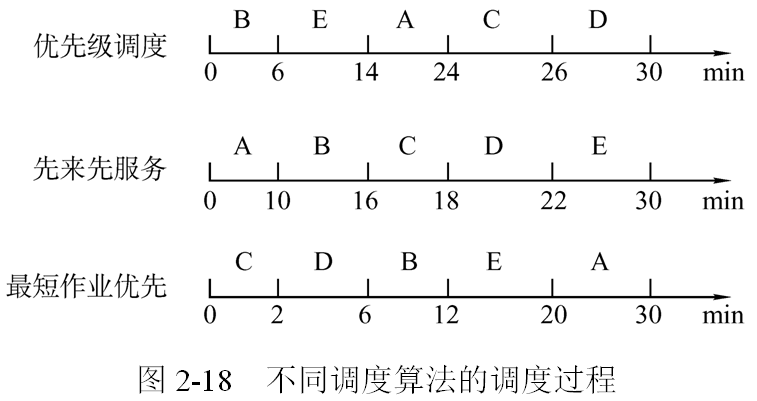
\includegraphics[width=2.42708in,height=1.28125in]{computerassets/D9AA33FBE58C25E01D7F0F0AA85BAC4D.png}
\end{solution}
